\NeedsTeXFormat{LaTeX2e}[2005/12/01]
%%    2010/04/06 v1.0 Vorlage Master-Forschungspraktikum Versuchsauswertung
%%    based on the 2009/10/14 v0.1 GAUBM template by Prof Pruschke

\documentclass[twoside,        %% zweiseitiges Layout
               BCOR12mm,       %% Bindekorrektur 12 mm
% please comment out if report is in English
%               english,ngerman, %% Dokumentspr. Deutsch, Alternativspr. Englisch
% please remove comment if report is in English 
               ngerman,english, %% Dokumentspr. Englisch, Alternativspr. Deutsch
               fleqn,headsepline=false,footsepline=false
              ]{Vorlage/MFPREPORT}
\makeatletter
\DeclareOldFontCommand{\rm}{\normalfont\rmfamily}{\mathrm}
\DeclareOldFontCommand{\sf}{\normalfont\sffamily}{\mathsf}
\DeclareOldFontCommand{\tt}{\normalfont\ttfamily}{\mathtt}
\DeclareOldFontCommand{\bf}{\normalfont\bfseries}{\mathbf}
\DeclareOldFontCommand{\it}{\normalfont\itshape}{\mathit}
\DeclareOldFontCommand{\sl}{\normalfont\slshape}{\@nomath\sl}
\DeclareOldFontCommand{\sc}{\normalfont\scshape}{\@nomath\sc}
\makeatother

%% Pakete und Definitionen ausgelagert
\usepackage{a4}
\usepackage{multicol}

% language option set in JGNSUM class
\usepackage{babel}
\usepackage{hyperref}

%% FONT:
%\usepackage{lmodern}
\usepackage{times} % sieht besser aus als lmodern
%\usepackage{palatino} % sieht schlechter aus als times
%\usepackage{mathpazo} % very ugly font, to be loaded later ???
%\usepackage{cmbright} % doesn't work either
\usepackage[T1]{fontenc}
\usepackage{textcomp}

\usepackage{ucs}
\usepackage[utf8x]{inputenc}

\usepackage{amsfonts}
\usepackage{amstext}
\usepackage{amsmath}
\usepackage{amsthm}
\usepackage{amssymb}
\usepackage{amsbsy}   % AMS-Boldsymbol

% \usepackage{mathabx} % e.g. for \Sun
%% but not a standard package (neither texlive nor Miktex)
%% so use wasysym (\astrosun) instead
\usepackage{wasysym} % e.g. for \astrosun or \CheckedBox

\usepackage{bbm,mathrsfs}

\usepackage{textcomp} % noch einige coole symbole

\usepackage{sectsty}
\allsectionsfont{\raggedright}

\usepackage[numbers]{natbib}
\citestyle{dinat}
\bibliographystyle{dinat}

\usepackage{makeidx}

\usepackage{url}	% für hübsche URLs mit Link
\usepackage{color}	% für farben a la \definecolor{Gray}{gray}{0.5}
\usepackage{verbatim}
\usepackage{subfigure}
\usepackage{listings}

\usepackage{fancybox}
%usage:
%\begin{Verbatim}[frame=single,label=Titel]
%Verbatim Zeile
%\end{Verbatim}


 \setlength{\textwidth}{16.2cm}
 \setlength{\textheight}{24cm}
 \setlength{\oddsidemargin}{0cm}
 \setlength{\evensidemargin}{-0.5cm}

 %unbedingt nach abmessungen einfügen!
 \usepackage{fancyhdr}
 \pagestyle{fancy}
 %\sloppy % für weniger absatzfehler

 \setcounter{tocdepth}{2}
 \setcounter{secnumdepth}{2}

 \ifreportelse{\numberwithin{equation}{chapter}}{\numberwithin{equation}{section}}
 \theoremstyle{plain}% default
 \ifreportelse{\newtheorem{thm}{Theorem}[chapter]}{\newtheorem{thm}{Theorem}[section]}

 \newtheorem{satz}{Satz}
 \newtheorem{lem}[thm]{Lemma}
 \newtheorem{prop}[thm]{Proposition}
 \newtheorem{kor}[thm]{Korollar}
 \newtheorem{cor}[thm]{Corollary}

 \theoremstyle{definition}
 \newtheorem{defi}{Definition}

 \def\@proof{%
  \if@englishpreamble{Proof}\else{Beweis}\fi
 }
 \newenvironment{bew}{\begin{proof}[\@proof]}{\end{proof}}



%% einbinden einiger nützlicher Befehle
\newcommand{\iflanggerman}[2]{
 \iflanguage{german}{#1}{
  \iflanguage{ngerman}{#1}{#2}
 }
}

% box around the whole equation, number inclusive
\newcommand{\boxedeqn}[1]{%
  \[\fbox{%
      \addtolength{\linewidth}{-2\fboxsep}%
      \addtolength{\linewidth}{-2\fboxrule}%
      \begin{minipage}{\linewidth}%
      \begin{equation}#1\end{equation}%
      \end{minipage}%
    }\]%
}

\iflanggerman{
 \newcommand{\const}{\mathrm{konst}}
 \newcommand{\Const}{\mathrm{konst.}}
}{
 \newcommand{\const}{\mathrm{const}}
 \newcommand{\Const}{\mathrm{const.}}
}

% von Meier
\newcommand{\nbd}{\nobreakdash-\hspace{0pt}}
% example: $K$\nbd{}Vektorraum
\newcommand*{\transpose}[1]{\prescript{t}{}{#1}}
\newcommand*{\conjugate}[1]{\overline{#1}}
\newcommand*{\abs}[1]{\lvert#1\rvert}
\newcommand*{\Mod}{\mathrm{mod}}
\newcommand{\symdif}{\mathbin\triangle}
\DeclareMathOperator{\Graph}{Graph}
\DeclareMathOperator{\id}{id}
\DeclareMathOperator*{\grad}{grad}
\DeclareMathOperator*{\Div}{div}
\DeclareMathOperator*{\rot}{rot}
\DeclareMathOperator{\sig}{sig}
\DeclareMathOperator{\sgn}{sgn}
\DeclareMathOperator{\diag}{diag}
\DeclareMathOperator{\tr}{tr}
\DeclareMathOperator{\Sp}{Sp}
\DeclareMathOperator{\im}{Im}
\DeclareMathOperator{\re}{Re}

\newcommand{\vcentcolon}{\mathop{:}}



%Zur Formatierung in der Matheumgebung
\renewcommand{\t}{\ensuremath{\rm\tiny}} % Tiefgestellter Text in der Matheumgebung wird schoener mit: $\Phi_{\t{Text}}$
\renewcommand{\d}{\ensuremath{\mathrm{d}}} % Die totale Ableitung ist stets aufrecht zu setzen: \d
\newcommand{\diff}[3][]{\ensuremath{\frac{\d^{#1}#2}{\d#3^{#1}}}} % einfache Ableitung nach x: $\ddx{\Phi}$
\newcommand{\pdiff}[3][]{\ensuremath{\frac{\partial^{#1}#2}{\partial#3^{#1}}}} % wie gesprochen, eine partielle Ableitung: \del
\newcommand{\aeqiv}{\ensuremath{\qquad \Longleftrightarrow \qquad}} % Eine Aequivalenz
\newcommand{\folgt}{\ensuremath{\qquad \Longrightarrow \qquad}} % Ein Folgepfeil mit Abstaenden
\newcommand{\corresponds}{\ensuremath{\mathrel{\widehat{=}}}} % Befehl für "Entspricht"-Zeichen
\newcommand{\mi}[1]{\ensuremath{\mathit{#1}}} % italics für griechische Buchstaben in Matheumgebung

%Um nicht so viel schreiben zu müssen...
\newcommand{\bs}[1]{\boldsymbol{#1}}
\newcommand{\ol}[1]{\overline{#1}}
\newcommand{\wtilde}[1]{\widetilde{#1}}
\newcommand{\mrm}[1]{\mathrm{#1}}
\newcommand{\mbf}[1]{\mathbf{#1}}
\newcommand{\mbb}[1]{\mathbb{#1}}
\newcommand{\mcal}[1]{\mathcal{#1}}
\newcommand{\mfrak}[1]{\mathfrak{#1}}

%Abkürzungen
\newcommand{\zB}{z.\,B.\ }
\newcommand{\bzw}{b.\,z.\, w.\ }
\newcommand{\Dh}{d.\,h.\ }
\newcommand{\Gl}{Gl.\ }
\newcommand{\Abb}{Abb.\ }
\newcommand{\Tab}{Tab.\ }

\usepackage{braket}
\usepackage{cleveref}
\usepackage{graphicx, subfigure}
\usepackage{rotating}
\usepackage{appendix}


\begin{document}
\LabratoryName{KT.HIP}{Higgs physics with the ATLAS experiment}
\ProtocolAuthor{Eric}{Bertok}{eric.bertok@stud.uni-goettingen.de}
\Assistant{K. Abeling}{}
\ResearchFocus{Nuclear and particle physics (M.phy.404)}
\ConductedOn{19}{04}{2018}
\date{\today}
% eines von beiden
\CopyNotWanted
%\CopyWanted

\pagenumbering{roman}
\maketitle

%\begin{otherlanguage}{english}
%\end{otherlanguage}

\tableofcontents

\clearpage
\pagenumbering{arabic}

\section{Introduction}
\label{sec:introduction}

\section{Theory}
\label{sec:theory}
\subsection{A summary of the Standard Model}
The Standard Model (SM) is the combination of different theories governing
three of the four known fundamental forces (electromagnetic, weak and strong
interactions), as well as all known elementary particles and their interaction. 
It consists of 6 quarks making up the hadrons, 6 leptons, as well as 4 gauge
bosons acting as force carriers for the interaction between the other
particles. The interactions are fixed by the principle of local gauge
invariance. The last puzzle piece - the Higgs boson - has recently been found at
the LHC. It gives mass to the other particles by the Higgs mechanism, a form of
spontaneous symmetry breaking. 
The Standard model has been a great success, having made predictions for new
physics as well as confirming these predictions with great accuracy. An example
of this is the theory of quantum-electro-dynamics, which has been confirmed to
an astounding precision [cite].
Despite the great success, the Standard Model is a rather ad-hoc combination of
different ideas without a unifying underlying theoretical principle. It
features 26 free parameters, namely the fermion masses, the coupling strengths
of the fundamental forces, mixing angles of quarks and neutrinos and parameters
specifying the Higgs mechanism \cite[p.\;500]{thomson}. Therefore, it is
desired that all four forces would unify into a ``Great Unified Theory'' (GUT).
There are other obvious shortcommings of the SM: Gravity is not
part of the SM, meaning that general relativity is not compatible with it,
although being much weaker than the other forces, it can be neglected in
particle experiments.
Furthermore, dark matter is not described by the SM. Furthermore, the
mass of the Higgs boson does not have the right mass order of magnitude at very
high energy scales due to loop corrections, a problem known as the ``hierarchy
problem'' \cite[p.\;505]{thomson}.

\subsection{Beyond the Standard Model}
Several ideas exist for an extension of the SM. Supersymmetry is an attempt to
both unify the electroweak and strong force as well as solving the hierarchy
problem. In supersymmetry, every elementary particle would have a corresponding
super-partner, called a ``sparticle''. So far, no super-partners have been
found \cite{thomson}. Also, there would be the need for 5 different Higgs
bosons. There is also a possibility of extra space-like dimensions that are
hidden from us, which would be a possible explanation for the weakness of
gravity. A prominent theory of quantum gravity - string theory - predicts these
extra dimensions. In an experiment, these extra dimensions could manifest as a
large amount of missing energy \cite{zwiebach2004first}. 
Additionally, neutrino masses need to be explained. A prominent idea is that
neutrinos are majorana particles, namely particles being their own
antiparticles.

\subsection{The Higgs mechanism}
\cite[Ch. 17]{thomson}
The Higgs mechanism is needed in the SM to give rise to massive gauge bosons
and fermions in a locally gauge invariant manner.
The problem can be illustrated with a simplified toy model. Consider a mass
term for a vector boson (e.g. a photon) in the Lagrangian:
\begin{align}
    \mathcal{L}_\text{mass}=\frac{1}{2}m_\gamma A_\mu A^\mu.
    \label{eq:massterm}
\end{align}
Such a term is not invariant under a local gauge transformation
\begin{align}
    \partial_\mu\rightarrow D_\mu&=\partial_\mu+i g A_\mu\\
    A_\mu\rightarrow A_\mu'&=A_\mu-\partial_\mu \chi(x).
    \label{eq:gauge}
\end{align}
One now introduces a complex scalar field $\phi(x)$ with a mexican hat
potential $V(\Phi)=\mu^2\phi^2+\lambda\phi^4$, which is shown in
\cref{fig:mexhat}. For $\mu^2<0$, $\lambda>0$, the potential minimum shifts
from the origin at $\phi=0$ to a degenerate ring in the complex plane. The
ground state thus chooses a new vacuum in an arbitrary direction with nonzero
$\phi$, a process called ``spontaneous symmetry breaking''. This ground state
can now be expanded around this minimum, choosing a convenient gauge, to
describe the system's low energy excitations in this new vacuum. This gives
rise to a massless particle called the Goldstone boson, as well a massive scalar
particle, called the Higgs boson. The original lagrangian expressed in this
gauge around this new minimum now has a mass term for the vector bosons without
having broken local gauge invariance.
The standard model Higgs has more subtleties arising from the noncommutativity
of the SU(2) and SU(3) gauge symmetries, but the general principle stays the
same.


\begin{figure}[]
    \centering
    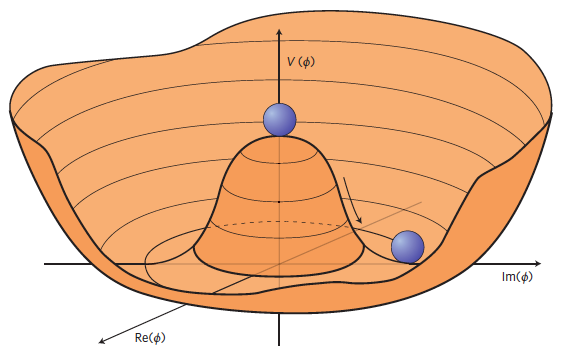
\includegraphics[width=0.5\textwidth]{fig/higgspotential}
    \caption{The mexican hat potential for the scalar Higgs boson. The
    symmetric state at $\phi=0$ is spontaneously broken and a new vacuum state
is chosen in a random direction. For a particular choice of ground state, the
low-energy excitations look like a massive scalar field in addition to a
massless Goldstone field. After a local gauge transformation, a mass term
for the vector bosons becomes visible in the lagrangian \cite{mexhat}.}
    \label{fig:mexhat}
\end{figure}

\subsection{Higgs decay and production}





\section{Experimental setup and methods}
\label{sec:setup}

\section{Analysis}
\label{sec:analysis}

\section{Discussion}
\label{sec:discussion}


\bibliography{literatur}
\newpage

\begin{appendices}
\end{appendices}

\end{document}

